\chapter{Event Reconstruction}
\label{cap4}
In the search of high mass in $W^+W^-$ channel, leptons (specifically, electrons or muons and neutrinos) and jets are searched for to select signal events.
The reconstruction of such objects follow standard algorithms and procedure which have been
developed by the experiment. In this chapter the reconstruction of the interested objects are described.

\section{The Particle Flow}
\label{PFt}
The algorithm for the events reconstruction is called Particle Flow (PF)~\cite{CMS-PAS-PFT-09-001}. It goals is to reconstruct all stable particle that emerging from a hadron-hadron collision, such muons, electrons, photons, charged hadrons and neutral hadrons. The PF technique uses the information coming from the 
CMS sub-detectors and combines them to obtain type of particle, their direction, the momentum and the energy.
The reconstruction of charged particles is allowed thanks to the presence of the silicon tracker that is immersed in the uniform magnetic field of 3.8 T. 
Thanks to that, a transverse momentum precise measurement could be done down to about 150 MeV.
The photon and electron reconstruction is performed by PF technique using the excellent tracking system together with he high granularity of the ECAL, this combination gives a high energy resolution for such particles.
The identification of charged-particles, energy clusters in the  calorimeters and muon tracks are the first step of the PF. All these information coming from sub-detectors and the information are then connected to each other making blocks of elements which are topologically compatible.
Starting by blacks, the candidates particle (PF Candidates) are fully reconstructed and identified as:
\begin{itemize}
\item Muons: the combination of a track in the tracker and a track in the muon system rise to a PF muon. The corresponding track is removed from the block after the identification.
\item Electrons: a charged-particle track is linked and one or more ECAL clusters (of presents)
\item Charged hadrons: PF charged hadrons give rise from the emaining tracks. Tracks can
be linked to ECAL and HCAL clusters, and the energy is determined taking into
account information from calorimeters.
\item Photons and Neutral hadrons:  a PF photons are given by a ECAL clusters not compatible with charged-tracks, instead PF
neutral hadrons are given by unaccounted HCAL deposits.
\end{itemize}
After that, once the list of PF Candidates is defined, the PF jets are clustered. At the end the PF MET is evaluated as the  opposite of transverse momentum-vector sum over all reconstructed PF Candidates.

\section{Tracking}
\subsection*{Hit reconstruction in the pixel and strip detector}
The first step of the reconstruction process is referred to as local reconstruction~\cite{Chatrchyan:2014fea}.  It consists of the clustering of zero-suppressed
signals above specified thresholds in pixel and strip channels into hits,  and then estimating the cluster positions and their uncertainties defined in a local
orthogonal  coordinate  system ($u$, $v$) in  the  plane  of  each  sensor (pixel and strip). 
The  hit reconstruction in the pixel detector and in the the strip detector is described below:
\begin{itemize} 
\item The pixel detector: in the data acquisition system of the pixel detector, zero-suppression is performed in the
readout chips of the sensors, with adjustable thresholds for each pixel.  This pixel readout threshold 
is set to a single-pixel threshold corresponding to an equivalent charge of 3200
electrons.  Offline, pixel clusters are formed from adjacent pixels, including both side-by-side
and corner-by-corner adjacent cells.  Each cluster must have a minimum charge equivalent to
4000 electrons.
\item The strip detector:  the clusters are seeded by any channel passing zero-suppression that has a charge at least a
factor of three greater than the corresponding channel noise. Neighbouring strips are added
to each seed, if their strip charge is more than twice the strip noise. 
A cluster is kept if its total charge is a factor five larger than the cluster noise.
The position of the hit corresponding to each cluster is determined from the charge-weighted
average of its strip positions, corrected for the  Lorentz drift.
\end{itemize}

\subsection*{Track reconstruction}
Different algorithms are used in CMS for track reconstruction,~\cite{Chatrchyan:2014fea, Adam:2005cg}.
All   methods   use   the   reconstructed positions (hits) of the passage of charged
particles inside the CMS silicon detectors to determine the
trajectories of the charged tracks and therefore measure their directions and momenta.  
The Combinatorial Track Finder (CTF) is the main standard algorithm and proceeds in three steps:
\begin{itemize} 
\item Seeding:  pairs of hits, that are compatible with the interaction region above a lower
$p_T$ limit, are considered as possible candidates of
charged tracks.  Pixel hits provide the best track
seeding, given their three-dimensional position in formation and lower occupancy.  
\item Finding: is based on a standard Kalman  Filter  pattern  recognition  approach.
The  track trajectory  is  extrapolated  to  the  neighboring tracker  layers, starting form the seeded parameters.
Compatible  hits  are  assigned to the track. 
The Kalman Filter, a  succession of  alternating  prediction  and  filtering  steps, 
updates the track parameters at each steps with new hits.
 The updated tracks are assigned a quality and only the best ones are kept for further propagation. 
\item Fitting: the  final  estimate  of  the   parameters  of
each  track  helix  is  completed  in  the  last  steps
applying again the Kalman Filter for the trajectory fitting.  Each trajectory is refitted using a
least-squares fit. In the central region, $|\eta|<1$, the $p_T$ resolution is better than 1\%  for tracks with $p_T<10\%$. At higher $p_T$ resolution worsens approximately as $\Delta (1/p_T) \sim 0.2$ TeV$^{-1}$.
\end{itemize}
The  reconstruction  of  single  muons  with  the
CTF  algorithm  is  almost  fully  efficient  over  the whole acceptance range.
Electrons, being charged particles, can be reconstructed through the standard track reconstruction.  However,  as electrons lose energy primarily through bremsstrahlung,  rather than ionization,  large energy losses are common.  
 The energy loss distribution is highly non-Gaussian, and therefore the standard Kalman filter is not appropriate.
Electron candidates are reconstructed using the  information from the tracker but also from
the ECAL, Sec~\ref{ler}. 
For charged hadrons the reconstruction is more problematic due to their nuclear
interactions  in  the  tracker  material. 


\subsection*{Primary-vertex reconstruction}
The goal of primary-vertex reconstruction~\cite{Speer:927395}  is to measure the location, and the associated
uncertainty, of all proton-proton interaction vertices in each event, including the ``signal'' vertex
and any vertices from pileup collisions, using the available reconstructed tracks.  
It consists of three steps: 
\begin{itemize} 
\item  selection of the tracks;
\item clustering of the tracks that appear to originate from the same interaction vertex;
\item fitting for the position of each vertex using its associated tracks.
\end{itemize}
Track selection involves choosing tracks consistent with being produced promptly in the primary interaction region, by imposing requirements on the maximum value of significance of the transverse impact parameter,  the number of strip and pixel hits associated with a track and the normalized
$\chi^2$ from a fit to the trajectory  ~\cite{Chatrchyan:2014fea}
The selected tracks are then clustered on the basis of their z-coordinates at their point of closest approach to the centre of the beam spot  using a
\textit{deterministic annealing} (DA) algorithm~\cite{726788}. 
The algorithm proceeds in a way that is analogous to that of a physical system approaching a state of minimal energy through a series of
gradual  temperature  reductions. 
The z-coordinates  of  the  points  of  closest  approach  of  the tracks to the centre of the beam spot are $z_i^T \pm \sigma_i^Z$.
 The tracks must be assigned to some unknown number of vertices at positions $z_k^V$.
The tracks can be associated with more than one vertex, with probability $p_{i,k}$ that is  the probability of the
assignment of track $i$ to vertex $k$ in a large ensemble of possible assignments.
 The most probable vertex positions at ``temperature'' T (like in the calculations in statistical mechanics) is,
\begin{equation}
F=-T \sum_{i}^{\# \; tracks} p_i \, \log \sum_{k}^{\# \, vertices} \rho_k  \exp [-\frac{1}{T} \frac{(z_i^T-z_k^V)^2}{(\sigma_i^z)^2}  ]
\end{equation}
 relative to the positions of the vertices $z_k^V$ with vertex weights $\rho_k$ (the weights are variable, but the sum is always constrained
to unity).
The DA algorithm is initiated at a very high temperature with a single vertex and $T$ is gradually decreased.
This procedure traces the global minimum of $F$ from high to low temperature.
The number of vertices increases as the temperature falls, and rises each time the minimum of $F$ turns into a saddle point at lower temperatures. 
The DA process thereby finds not only positions and assignments of tracks to vertices but also the number of vertices.
In Fig.~\label{Fig:pu} is shown the distributions of the number of vertices in a Drell-Yan sample.
\begin{figure*}[htbp]
\centering
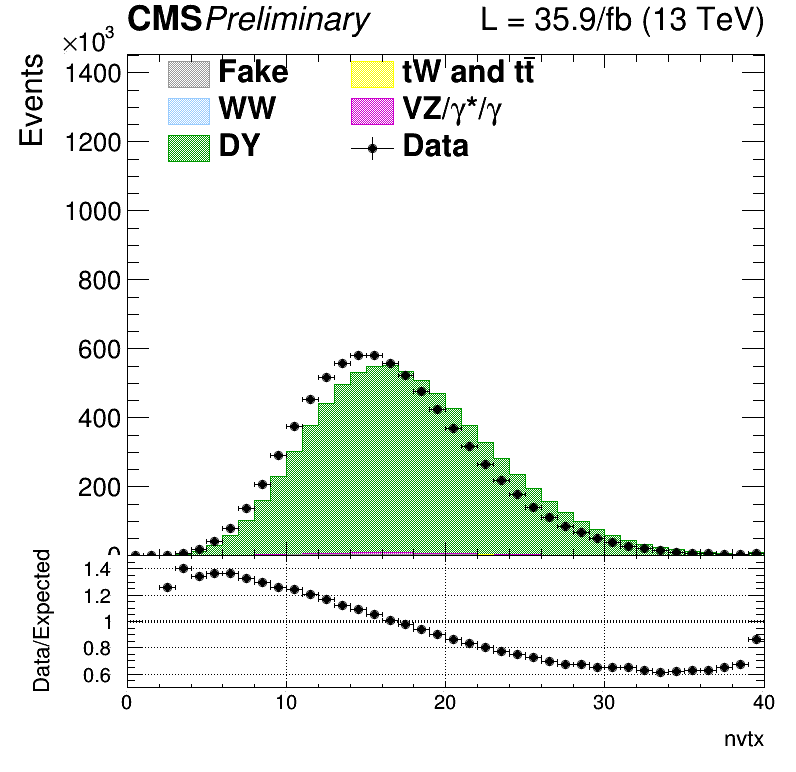
\includegraphics[width=0.6\textwidth]{../AN/Figs/nvertices.png}
\caption{
    Distributions of the number of vertices in a Drell-Yan enriched sample
    (Z$\rightarrow{}ee$) in
    data}
    \label{Fig:pu}
\end{figure*}




\section{Calorimeter clusters}
The purpose of the clustering algorithm in the calorimeters are~\cite{Sirunyan:2017ulk}:
\begin{itemize} 
\item detect and measure the energy and direction of stable neutral particles such as photons and neutral hadrons;
\item separate these neutral particles from charged hadron energy deposits;
\item reconstruct and identify electrons and all accompanying bremsstrahlung photons;
\item help the energy measurement of charged hadrons for which the track parameters were not determined accurately,
which is the case for low-quality and high $p_T$ tracks.
\end{itemize}
For the PF event reconstruction, a  specific clustering algorithm was developed. 
The clustering is performed separately in each subdetector: ECAL (barrel and endcaps) and HCAL (barrel and endcaps)
In the algorithm, first, \textit{cluster seeds} are identified   as cells with an energy larger than a given seed threshold, and
larger than the energy of the neighbouring cells. Second, \textit{topological clusters} are grown from the seeds by aggregating cells with at least a corner in common with a cell already in the cluster.
After an expectation-maximization algorithm based on a Gaussian-mixture mode to
reconstruct the clusters within a topological cluster is used.
The Gaussian-mixture model postulates
that the energy deposits in the M individual cells of the topological cluster arise from N Gaussian energy deposits where N is the number of seeds. 
The expectation-maximization algorithm is an iterative algorithm with two steps at each iteration.
During the first step, the parameters of the model are kept constant and the parameters of the model are determined during the second step in an analytical maximum-
likelihood. 
The energy and position of the seeds are used as initial values for the parameters of the corresponding 
Gaussian functions and the expectation maximization cycle is repeated until convergence.

\section{Link algorithm}
A given particle is, in general, expected to give rise to several PF elements in the various CMS
subdetectors. The reconstruction of a particle therefore first proceeds with a
link algorithm that connects the PF elements from different subdetectors.
The link between a track in the central tracker and a calorimeter cluster is established:
the track is first extrapolated from its last measured hit in the tracker to
 the ECAL at a depth corresponding to the expected maximum of a typical longitudinal electron shower
profile, and to the HCAL at a depth corresponding to one interaction length.  
The track is linked to a cluster if its extrapolated position is within the cluster area, defined by the union of the
areas in the HCAL and the ECAL in $(\phi, \eta)$ plane. 
After, Calorimeter cluster-to-cluster links are sought between HCAL clusters and ECAL clusters.
Charged-particle tracks may also be linked together through a common secondary vertex, for
nuclear-interaction reconstruction.
Finally, a link between a track in the central tracker and information in the muon detector is
established to form global and tracker muons, Sec~\ref{ler}.\\

In each PF block, the identification and reconstruction sequence proceeds as,
\begin{itemize} 
\item first, muon candidates are identified and reconstructed and the
corresponding PF elements (tracks and clusters) are removed from the PF block.  
\item The electron identification and reconstruction follows. Energetic and isolated photons, converted or un-
converted, are identified in the same step.  The corresponding tracks and ECAL or preshower
clusters are excluded from further consideration
\item The remaining elements in the block are then subject to a cross-identification of charged hadrons,
neutral hadrons, and photons, arising from parton fragmentation, hadronization, and decays
in jets. 
\end{itemize}

\section{Jet Energy Calibration}
The purpose of the jet energy calibration is to relate, on average, the energy measured for the
detector jet to the energy of the corresponding true particle jet.  A true particle jet results from
the clustering (with the same clustering algorithm applied to detector jets, Sec.~\ref{jetr}) of all stable particles
originating from the fragmenting parton, as well as of the particles from the underlying event
(UE) activity. 

The jet energy calibration is related,  on average, on the energy measured in
the detector to the true energy of the corresponding final state particle jet or parton jet.
From the clustering  of all stable particle, a true particle jet results. The correction is applied as
a multiplicative factor C to each component of the raw jet four-momentum vector, $p_{\mu}^{raw}$, as:
\newline
\begin{equation}
p_{\mu}^{corr}=C \cdot p_{\mu}^{raw} \; ,
\end{equation}
where correction factor $C$ is composed of the offset correction $C_{offset}$ , the MC calibration
factor $C_{MC}$, and the residual calibrations $C_{rel}$ and $C_{abs}$ for the relative and absolute
energy scales, respectively. The various components are applied in sequence:
\newline
\begin{equation}
C=   C_{offset} ( p_{\mu}^{raw}) \cdot  C_{MC} (p_T',\eta) \cdot C_{rel}(\eta) \cdot  C_{abs} (p_T'') \; ,
\end{equation}
\newline
where $p_T'$ is the transverse momentum of the jet after applying the offset correction and $p_T''$ is the transverse momentum 
of the jet after all previous corrections. The details of each component are:
\begin{itemize}
\item $C_{offset}$: a energy offset is produced by the pileup of multiple proton-proton collisions and by electronic noise.
The goal of the offset correction is to subtract, on average, the unwanted
energy from the jet. For the offset correction estimation, the Jet Area Method has been used. 
An average $p_T$-density $\rho$ per unit area is estimated, for each event. 
The key element for this approach is the jet area $A_j$.
A very large number of infinitely soft four-momentum vectors are artificially added in the event and clustered
by the jet algorithm together with the true jet components. The other important quantity for the pileup subtraction is the $p_T$ density $\rho$, which
is calculated with the $k_T$ jet clustering algorithm with a distance parameter R$=$0.6.
The quantity $\rho$ is defined on an event-by-event basis as the median of the distribution of
the variable $p_{Tj}  /A_j$ , where j runs over all jets in the event, and is not sensitive to the
presence of hard jets. Therefore, the event-by-event and jet-by-jet offset correction can be defined as,
\begin{equation}
  C_{offset}= (p_T^{raw}, A_j ,\rho )=1- \frac{(\rho -\langle \rho_{UE}  \rangle )\cdot A_j }{p_T^{raw}} \; ,
\end{equation}
where $\langle \rho_{UE}  \rangle$ is the $p_T$-density component due to the UE and electronics
noise, and is measured in events with exactly one reconstructed primary vertex (no pileup).
\item $C_{MC}$: is based on the simulation and corrects the energy of the reconstructed
jets such that it is equal on average to the energy of the generated jets (GenJets). The
GenJets reconstruction algorithm is identical to the one applied to the data.
The response variable, $R=p_T^{reco}/p_T^{gen}$, in each bin of the GenJet transverse momentum $/p_T^{gen}$, is recorded as jet $p_T^{reco}$.
The average correction in each bin is defined as,
\begin{equation}
  C_{MC}(p_T^{reco})= \frac{1}{\langle R \rangle } \; ,
\end{equation}
\item $C_{rel}$: the goal of the relative jet energy scale correction is to make the jet response flat versus $\eta$. 
This is achieved by employing a Tag and Probe technique, selecting dijet
events in data. The size of this residual correction is of the order of 2-3\% in the
central $\eta$ region, while it goes up to about 10\% in the forward region.
\item $C_{abs}$: the goal of the absolute jet energy scale correction is to make the jet response flat versus $p_T$.
Once a jet has been corrected for $\eta$ dependence, it is corrected back to particle
level.
\end{itemize}
Each type of correction has uncertainties arising from many different sources.
These sources are categorized as: physics modeling in MC, MC modeling of true detector response and potential biases in the methodologies used to estimate the corrections. In CMS more than 16 such sources of uncertainties have been identified. Several are
related and can be combined into groups that are relative to the absolute scale, relative
scale, extrapolation in $p_T$ , pileup, jet flavor and time stability.

\section{Pileup subtraction}
At the LHC,  at each bunch crossing there are of the order of 20 minimum bias proton-proton interactions, which pollute any interesting hard events with many soft particle. The kinematic measurements for jets will be adversely affected by pileup (PU), with resolution and absolute energy measurements
suffering significantly: in fact for the  neutral particles is not possible distinct primary vertex that corresponds to a single
proton-proton interaction,  and most jet measurements are carried out with calorimeters, which do not have the angular
resolution needed to reconstruct the original primary vertex.\\
An event-by-event, and jet-by-jet, pileup subtraction approach, which performs the corrections after the jet finding,  has been
carried out~\cite{Cacciari:2007fd}.  It is based on:
\begin{itemize}
\item the jet’s susceptibility to contamination: it is embodied in the jet area A measured on $\eta$ and $\phi$. The jet area is different for each jet and depends on the details of its substructure, and practical measurement of the jet areas is carried out using the FastJet package. 
Given a suitable definition of jet area, the modification of a jet’s $p_T$ by diffuse noise can be shown to be,
\begin{equation} 
\Delta p_T=A\rho \pm \sigma \sqrt{A} -L \:, \qquad \langle L \rangle=\mathcal{O}(\alpha_S \times A \rho \ln \frac{p_T}{ A \rho}) \:,  
\end{equation} 
where $\rho$ is the level of diffuse noise that  corresponds to the amount of transverse momentum added to the event per unit area (at LHC is around 
10-20 GeV~\cite{Sjostrand:2003wg}): the first term is therefore the geometrical contamination of the jet 
and is associated with an uncertainty (second term) because of fluctuations in the noise from point to point in the event.
$L$  accounts for the occasional loss (or the even more occasional gain) of part of the jet’s contents,
due to the fact that jets can be modified when clustered in the presence of diffuse noise, as some
of the particles originally clustered into one jet can instead end up in a different one. \\
If the fluctuations are small, $\sigma << \sqrt{A} \, \rho$, the measured $p_T$ for each jet $j$ using the subtraction is given by,
\begin{equation} 
p_{T,j}^{sub}=p_{T,j} -A_J \rho \: ,
\end{equation} 
where $A_j $ is the jet area. This equation provides a correction to the jet’s scalar transverse
momentum.
\item The second ingredient in carrying out the subtraction is the estimate of $\rho$ for each event.
The principal difficulty in estimating the amount of noise is that of distinguishing the noise component from the large amounts of $p_T$ deposited by the hard event.
The $\rho$ value  for each even can be estimated~\cite{Cacciari:2007fd}  taking the median value of this distribution in the event: 
\begin{equation} 
\rho= median \; [\{\frac{p_{T,j}}{A_j}\}]  \: ,
\end{equation} 
\end{itemize}
The above pileup subtraction procedure is valid if: 
\begin{itemize}
\item The pileup noise should be independent of $\eta$ and $\phi$.
\item The radius $R$ of the jet algorithm should be no smaller than the typical distance between minimum bias particles, otherwise the extraction of
 $\rho$ from the median will be biased by the large amount of empty area not associated with jets
\item The number of pileup jets should be much larger than the number of jets from the hard interaction. 
\end{itemize}



\section{Lepton reconstruction and identification}
\label{ler}
\subsection*{Electron reconstruction and identification}
The combination of tracker and ECAL information is used for electrons reconstruction.
The electrons, emerging from a collision, when interact with the silicon tracker, radiate bremsstrahlung photons that reaches the ECAL with a significant spread in the azimuthal direction $\phi$. These energy deposited measured in ECAL are the starting point of the electrons reconstruction algorithm. The energy deposited are associated clusters and in superclusters (clusters of clusters) that take into account the spread in  $\phi$ direction of the bremsstrahlung energy, Fig.~\ref{clustering}.
When   superclusters are identified, the reconstruction algorithm tries to match them to track seeds. The  track seeds are identified as pairs or triplets of hits in the inner tracker layers. The electrons trajectories are reconstructed using a dedicated modeling that take in account  energy
loss in the tracker layers via  bremsstrahlung radiation. In general, non-Gaussian contributions to the event-by-event fluctuations 
of the calorimetry and tracking measurements, are introduced due to the  bremsstrahlung radiation.   electron candidates are reconstructed using 
\begin{figure}
\centering
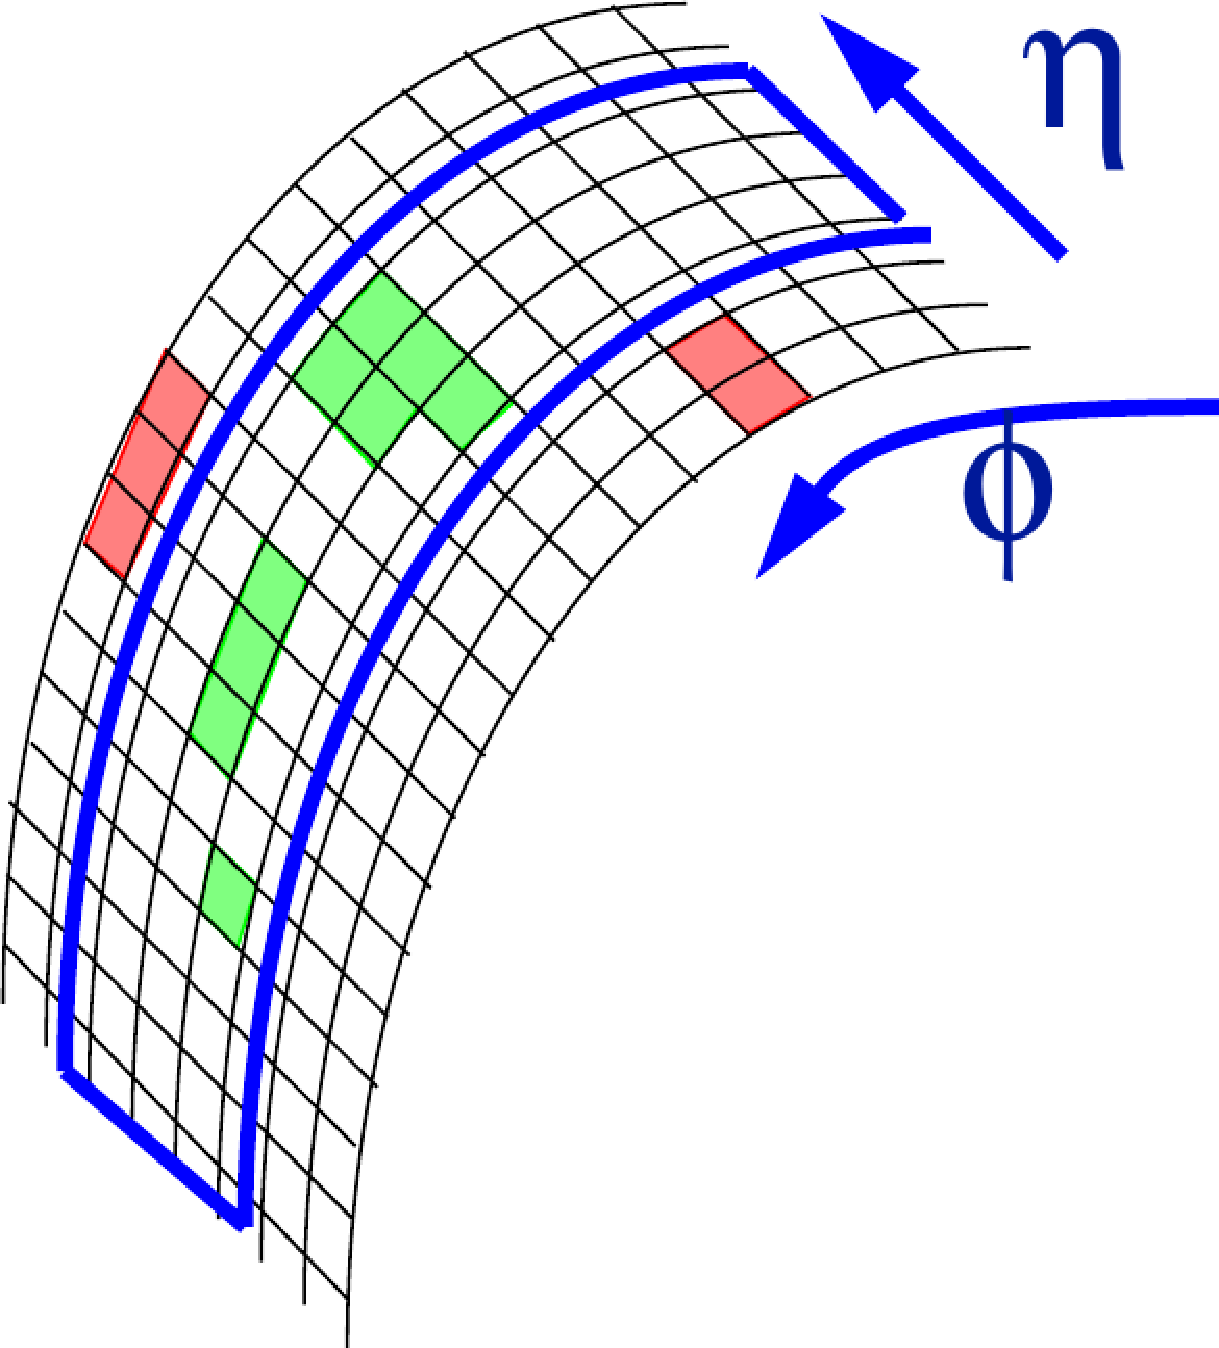
\includegraphics[scale= 0.2]{../Cap4/clustering}
\caption{Cluster spread in $\eta$ and $\phi$.}
\label{clustering}
\end{figure}
A preselection is applied to solve ambiguous cases where several tracks are reconstructed. Is is based on matching
between the GSF track and the supercluster in $\eta$ and $\phi$.To perform a good resolution electron supercluster must
be inside the ECAL acceptance volume, that meaning  $\eta<$ 2.5 and outside the ECAL barrel-endcap
overlap region, 1.4442 $<\eta<$ 1.566.
Several identification variables are used to achieve a good discrimination. These variable are:
\begin{itemize}
\item $\Delta \eta_{trk,SC}$ and $\Delta \phi_{trk,SC}$, that measurements the spacial matching between the track
and the supercluster.
\item $\sigma_{in,in}$ that measurs the width of the ECAL supercluster in the $\eta$ direction. It is calorimeter shower shape.
\item H/E: is is the ratio among the energy deposit in the HCAL tower and the energy of the seed supercluster.
\item $|$1/E - 1/p$|$ the difference of 1/E measured in ECAL and the 1/p measured in the tracker.
\item Number of missing hit
\item $d_{xy}$ and $d_z$, impact parameters respect to the reconstructed primary vertex (PV).
\item $\gamma \to e^+ e^-$ veto based on missing hits in the inner layers of the tracker.
\end{itemize}
Different selections on the previously variables defined different working points. The cuts are different for electrons in
the ECAL barrel or in the endcap. These are defined below:
\begin{itemize}
\item Tight WP: this corresponds to an average 70\% selection efficiency for electrons with
$p_T >$ 20 GeV. this working point is used where backgrounds are very large. The
$X \to WW$ high mass analysis has large backgrounds like W+jets, where the second lepton is fake. 
So, in this analysis we use Tight WP for electrons. On the top of that, we apply more cuts to make the electron id selection Trigger safe.
\item Medium WP: the average efficiency is about 80\% for electrons with $p_T>$ 20
GeV. This is also a good starting point for measurements of W and Z cross-sections.
\item Loose WP: this working point is used only for very clean final states. The average efficiency is about 90\%.
\item Veto WP: generally, this is not used for signal selection. However, it is found to
be useful for extra lepton veto counting of electrons. The average efficiency is about 95\%.
\end{itemize}
The electrons selected, are also required to pass the isolation criteria that including a pile-up mitigation correction based on the electron effective 
catchment area. The isolation variable is computed for each electron as,
\begin{equation}
ISO^{Rel}_{EA\; corrected}=[\sum_{ChH}(p_T) + max(0, \sum_{Ph}(p_T)) +\sum_{NH}(p_T)  -\rho EA ]/p_T^{electron} \, ,
\end{equation}
where $ChH$ is the charged hadrons, $Ph$ is photons, $NH$ is neutral hadrons, $\rho$ is the pile up energy
density and $A$ is an effective area. The sums are in a isolated cone of $\Delta R<$ 0.4 around the electron direction.
The identification and isolation criteria used for the $X \to WW$ analysis are reported in Tab.~\ref{IDe}.

\begin{table}
\centering
\begin{tabular}{|lll|}
\hline
Observable & Barrel (EB) cut &Endcap (EE) cut\\
\hline
$|\Delta \eta_{trk,SC}|$  &0.00308  & 0.00605 \\
$|\Delta \phi_{trk,SC}|$ & 0.0816   &0.0394\\
$\sigma_{in,in}$ &0.011& 0.031\\
H/E & 0.060& 0.065\\
$|$1/E - 1/p$|$ & 0.013 &0.013\\
Number of missing &1&1\\
$|d_{xy}|$ &0.05&1\\
$|d_z|$ &1&1\\
conversion veto& true&true\\ 
\hline
$ISO^{Rel}_{EA\; corrected}$&0.0588 & 0.0571\\
\hline

\end{tabular}
\caption{Electron identification for Tight working point  and isolation requirements.}
\label{IDe}
\end{table}

\subsection*{Muon reconstruction and identification}
Muons are produced in the interaction point and they can pass all the detector with a negligible energy loss, given a signal in the muon chamber.
Their loss of energy is very negligible. 
Muons are thus reconstructed both in the silicon tracker and in the external muon chambers. 
The reconstruction starts from the measurements of DT, CSC and RPC sub-detectors. The reconstructed track in the muon spectrometer is called
Stand-alone Muon.
In the inner silicon tracker the muon track are also reconstructed. Seeds are
built using two or three consecutive hits in the pixel and or in the strip detector. 
The pattern recognition is performed starting from these seeds and proceeding layer by layer,
with an iterative technique based on the Kalman Filter technique.
At the end of this algorithm, a track fit is performed and the track parameters are updated. The identified
tracker track is then combined with a given Stand-alone Muon track in order to construct
a global track, which defines a Global Muon. A global fit is performed for each pair of
tracks reconstructed in the inner tracker and in the muon system. If more than one track
matching the stand-alone track is found, then the one giving the best $\chi^2$ in the global fit
is chosen. Exist a second approach that consists in considering all tracker tracks with $p_T>$ 0.5 GeV as
potential muon candidates. These tracks are extrapolated to the muon system taking
into account the magnetic field. If at least one muon segment (a short track stub made of
DT or CSC hits) matches the extrapolated tracks, the corresponding tracker track is
identified as a Tracker Muon.
Quality requirements are applied to ensure a good quality of the reconstruction:
the tracker track has to be reconstructed from at least 5 tracker layers with hits;
\begin{itemize}
 \item at least one hit must be present in the pixel detector;
 \item least one hit must be present in the muon detector;
 \item least one muon chamber hit should be included in the Global Muon track fit;
 \item normalized $\chi^2$ of the Global Muon track fit should be less than 10;
 \item muon track reconstructed in the tracker must have a distance to the primary
vertex (PV) smaller than 2 mm in the transverse plane and smaller than 5 mm in
the longitudinal direction.
\end{itemize}
The requirements are summarized in Tab.\ref{IDm}

\begin{table}
\centering
\begin{tabular}{|ll|}
\hline
Observable& Value Cut\\
\hline
Is global muon                        & true              \\ 
Is PF muon                            & true              \\ 
Tracker layers with measurements      & $>5$              \\ 
Number of valid pixel hits            & $>0$              \\ 
Number of valid muon hits             & $>0$              \\ 
Number of matched muon stations       & $>1$              \\ 
$\chi^2$ /ndof                        & $<10$             \\ 
$d_{xy}$ (PV)                         & < 0.2 cm          \\ 
$d_z$ (PV)                            & < 0.5 cm          \\ 
\hline
\end{tabular}
\caption{Muon identification and isolation requirements..}
\label{IDm}
\end{table}
For the analysis goals, the muon are expected to be isolated, as the  produced by W boson decay. Indeed, prompt muons are expected to be isolated in the event, contrary to non-prompt muons that are generally produced within jets and characterized by many
nearby particles. Muon coming from $W$, and so from $X$, must be isolated and they are requested to pass an isolation
criterion which also icludes a PU mitigation correction called ``$\Delta \beta$ correction''.
The isolation variable is therefore sensitive to the
pileup and a correction is needed in order to ensure its independence and robustness on
the number of simultaneous interactions. The isolation variable used is,
\begin{equation} 
ISO^{Rel}_{\Delta \beta}=[\sum_{ChH}(p_T) + max(0, \sum_{Ph}(p_T) -0.5 \times \sum_{ChHUP}(p_T)) ]/p_T^{electron} \, ,
\end{equation}
where $ChH$ is the charged hadrons, $Ph$ is photons and $ChHPU$ is charged
hadrons not coming from the primary vertex.  The sum is performed in a cone of 0.4 units in $\Delta R$ around the muon.
A bias in the muon $p_T$ is introduced by the imperfect knowledge
of the magnetic field and the effect of the material distribution. In addition the $p_T$ measurement is sensitive to the alignment of the tracker and
muon chambers. To estimate the muon $p_T$ scale and resolution are used different method. For $p_T<100$ GeV, the  events with two muon arising from the $J/\Psi$ and Z
resonance decays are used to correct the $p_T$ scale. Above, so in the high $p_T$ regime, are used cosmic ray muons.

\section{Jet reconstruction and identification}
\label{jetr}
Jets are the experimental signature of quarks and gluons produced in the hadron collision. They result from the parton  hadronization and they play a major in a hadronic collider where final state with jets have very large cross-section. The technique used for jet reconstruction is the Particle Flow.
Using the particle-flow algorithm described in Sec.~\ref{PFt}, the  jets are reconstructed by clustering of the  four-momentum vectors of candidates: the information from relevant CMS sub-detectors are used to identify and to reconstruct all visible particles in the event, as
 muons, electrons, photons, charged hadrons, and neutral hadrons. 
The momentum and spatial resolutions of jet identified with PF technique, are greatly improved respect to jet identified with only the calorimeter information. Indeed the use of the tracking detectors allows a better resolution of $p_T$ for the charged particles.
The sequential and iterative jet clustering algorithm, that combine four-vectors of input particles, are used to form the jets.
A ideal jet clustering algorithm should have the following features:
\begin{itemize}
\item infrared safety: infrared singularity should not appear in the perturbative calculation;
\item collinear safety: collinear singularities must not appear in the perturbative calculations;
\item invariance under boosts: the algorithm should find the same solutions independently
by boosts in the longitudinal direction.
\item order independence: the algorithm should find the same jets at parton, particle, and detector level;
\item straightforward implementation: the algorithm should be straightforward to imple-
ment in perturbative calculations.
\end{itemize}
The jet algorithm should also follow these  experimental criteria
\begin{itemize}
\item detector independence: the performance of the algorithm should be as independent from the detector;
\item minimization of resolution smearing and angle biases: the algorithm should not
amplify the inevitable effects of resolution smearing and angle biases;
\item stability with luminosity: jet finding should not be strongly affected by pileup;
\item efficient use of computing resources: minimum of computer time consumption;
\item maximal reconstruction efficiency: the algorithm should efficiently identify all jets;
\item ease of calibration and use: algorithm should not obstruct to the reliable calibration and and to be straightforward to implement.
\end{itemize}
Jet definition is not unique, being the parton not a well-defined object, so several
approaches for jet clustering are available. Two main algorithms for clustering have been developed. The ``conical recombination''
where jets are defined as dominant directions of energy flow.  The second class is called sequential recombination and it works by defining a distance
between pairs of particles, performing subsequent recombinations of the pair of closest
particles and stopping when all resulting objects are too far apart. The standard algorithms adopted by
CMS are the SISCone in the conical recombination class, and the $k_t$, Cambridge-Aachen (CA) and anti-$k_T$ algorithms, Sec~\ref{rico_jet}.\\
\newline

\subsection*{Jets in $X \to WW$}
The jets collection is made by clustering the reconstructed particles known as the Particle Flow
Candidates in the CMS software. The reclustering algorithm used is the anti-kt algorithm with
a distance parameter equal to 0.4. Pileup mitigation is done with the Charge Hadron Subtraction  algorithm 
which removes charged particles coming from pileup vertices before
clustering.
The Jet Energy Corrections  that are applied to correct the reconstructed jet energy back
to the true energy of the final state particles.  To reject jets originating
from calorimeter or readout electronics noise the loose working point of the PF Jet Identification is applied. 
This analysis selects a jet by the selection cut as,
\begin{equation}
 p_T^{Jet} > 30 GeV \: , |\eta| < 5.0 \: .
\end{equation}
The various distributions of jet after correction are shown at Fig.~\ref{jetFig}
\begin{figure}
\centering
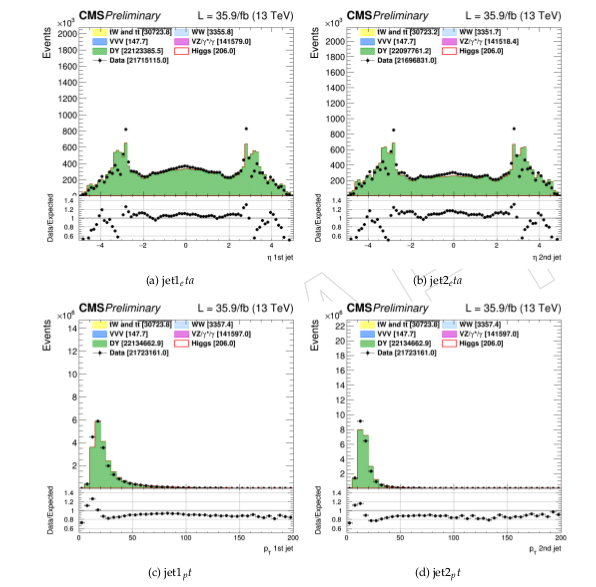
\includegraphics[scale= 0.5]{../Cap4/jetFig}
\caption{The jet kinematic distributions:.}
\label{jetFig}
\end{figure}

\section{b-jet identification}
To identify the b jets  the properties that characterize hadrons are used
containing the quark b.
In fact these hadrons have a relatively large mass, around 5 GeV, and a long average life, about 1.5 ps. Given that they can
have an impulse of several tens of GeV, the distance that they travel in the detector
it is of the order of:
\begin{eqnarray}
\delta &\approx& t_{medio} \: v \approx \gamma \: \tau \: \beta  \: c  \nonumber \\
 &\approx& 10 \cdot 1.5 \cdot 10^{-12} \mbox{s} \cdot 1 \cdot 3 \cdot 10^8 \: \mbox{m/s}   \nonumber \\
 &\approx& 5  \mbox{mm.} \end{eqnarray}
A distance that can be measured since the accuracy of the position of the
secondary vertices is $\sim$100 $\mu$m.
The CMS collaboration has developed different algorithms to identify the jets coming from
  quarks b (b-tag algorithms). Each of these algorithms is characterized
from a certain efficiency of signal identification (jets from b quark) and from the probability of
reject the background (jet not from b quark), which in general depend on the transverse impulse,
$p_T$, and from the pseudorapidity  of the jet. To build an observable (or discriminator) which distinguishes 
the jets originated by b from those originating from light quark 
is used to reconstructed objects such as, traces, vertices and leptons. 
Some algorithms simple but reliable use a single observable in input, while others
more complexes combine different ones to generate the discriminator. Each algorithm
produces, in output, a single value of the discriminator for each jet of the event.
The first step in identifying of b-jets is the reconstruction of all the jets present in the
the event. As mentioned, the CMS collaboration uses for jet reconstruction
the anti-$k_T$ algorithm, applied to Particle Flow objects. However the algorithms of
identification require a sample with well reconstructed and high purity traces.
Therefore further cuts to the traces of the jet are applied. First of all, to reduce
the number of traces reconstructed incorrectly, a transverse pulse is required
greater than 1 GeV and at least two signals in the silicon pixel detector. Then, at 
least eight signals per track must be present with a fit that has a
 $\chi^2$/d.o.f. $<$5, where d.o.f. it is the number of degrees of freedom of the fit. It also applies
also a selection on the impact parameters: this is used to increase
the fraction of well reconstructed traces and to reduce the contamination due to long life particles like neutral kaons.
The transverse distance $d_{xy}$ and longitudinal $d_z$ between the trace and the primary vertex
are required to be smaller than 0.2 cm and 17 cm respectively.
In Fig.~\ref{bj}  it is
was a schematic representation of the parameters used in the identification
of the b jets.
\begin{figure}
\centering
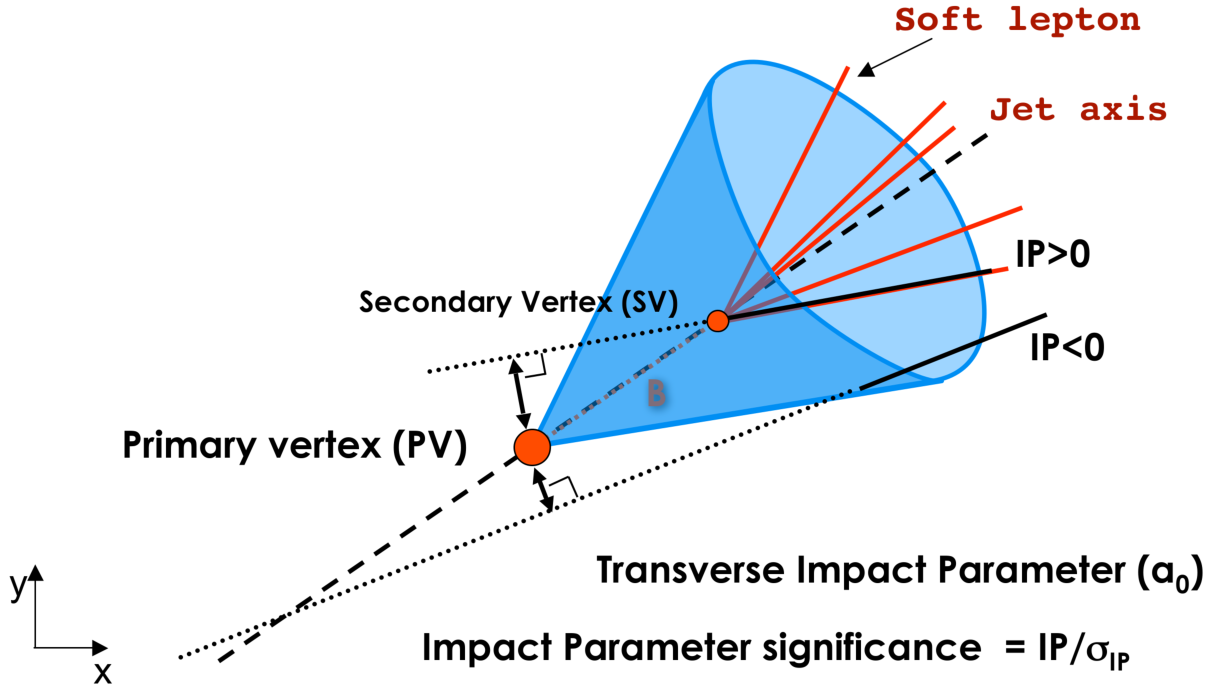
\includegraphics[scale= 0.5]{../Cap4/btag}
\caption{Cluster spread in $\eta$ and $\phi$.}
\label{bj}
\end{figure}
\subsection*{Impact Parameter algorithm}
The impact parameter (IP) of a track respect to the primary vertex, can be used to distinguish 
the hadrons b decay  respect to background tracks (prompt). The IP is calculated in three dimensions 
thanks to the excellent resolution of the pixel detector.
The impact parameter has the same sign of the product scalar between the direction of the
jet and the distance of the primary vertex from the nearest point of the trace. The traces
produced by particles due to the decay of a hadron with a long average life
they have a positive value of IP, while for the traces originated from the primary vertex
(prompt) the IP will be both negative and positive.
The variable used as observable is the significance of the parameter of
pact, S$_{IP}$, defined as the relationship between IP and its estimated uncertainty. There
significance of the impact parameter can therefore be used as a discriminant  between b and non-b jets.
The Track Counting (TC) algorithm orders in significance
IP traces of jets, from the highest to lowest. There are two different versions of this algorithm that
they are distinguished on the basis of which significance value is taken into consideration:
Track Counting High Efficiency (TCHE) uses the S$_{IP}$ of the second track , while the Track Counting High Purity (TCHP) use the third.
A natural extension of the TC algorithms is the combination of the several tracks impact points. 
This is implemented in the Jet Probability (JP) and Jet algorithms
B Probability (JBP). The former uses an estimator for the likelihood he evaluates
which may be the probability that all traces associated with a jet come from
from the vertex of primary interaction. The estimator of likelihood, P$_{jet}$, is defined
such as,
\begin{equation}
P_{jet}=\Pi \cdot \sum_{i=0} ^{N-1} \frac{(-\ln \Pi)^i}{i!} \qquad \mbox{con} \qquad \Pi= \prod_{i=0} ^{N}\mbox{max}(P_i, 0.005)  \mbox{,}\end{equation} 
where N is the number of traces considered and P  the probability that the track is
originated in the primary vertex.
Instead the JBP algorithm gives more weight to the tracks (up to a maximum of four) than
they are connected to a jet from b; these are identified as they have a high level
value of the significance of IP.

\subsection*{Secondary Vertex identification}
The presence of a
secondary vertex in the event and related variables  can be used
to discriminate jets coming from a quark b respect to the others. The main variables associated with the secondary vertex are the distance, the flight direction
with respect to the primary vertex, the mass and the energy of the particles associated to the traces
secondary. To identify a secondary vertex it is required that:
\begin{itemize}
\item shares less than 65\% of its traces associated with the primary vertex and
the significance of the radial distance between the two vertices is beyond 3$\sigma$;
\item the flight distance of each candidate is in a cone with $\Delta R <$0.5 around
to the direction of the jet;
\item the secondary candidates who have a distance over
per 2.5 cm above the primary vertex, both a mass compatible with
that of K$_0$ or that in any case exceeds 6.5 GeV.
\end{itemize}
The Simple Secondary Vertex (SSV) algorithm uses as a discriminating variable 
the significance of the flight distance, given by the distance ratio of
flight with its uncertainty. Similar to the TC algorithm, there are two versions
of SSV: High Efficiency (SSVHE) which uses vertices to which they are associated at least
two tracks, and High Purity (SSVHP) that requires at least three tracks.
There are more complicated algorithms that consider the secondary vertices together with the
information on the average life. This makes it possible to construct a discriminant
even when there is no secondary summit, increasing efficiency in terms of
to SSV; two of these algorithms are the Combined Secondary Vertex (CSV) and the
Combined Secondary Vertex Version 2 + Inclusive Vertex Finder (CSVV2IVF).
The difference between the two is that the CSV algorithm uses to reconstruct the vertices share information from jets while the CSVV2IVF algorithm uses
all the tracks present in the event.
Moreover, in general, there are some variables that are not very related to each other and that
they can be used as good discriminators that are:
\begin{itemize}
\item the category of vertices;
\item the significance of the flight distance in the transverse plane;
\item the mass of the vertex;
\item the number of vertex tracks;
\item the ratio between the energy carried by a track and the other jet tracks;
\item the pseudorapidity of the track;
\item the number of traces in the jet.
\end{itemize}

\subsection*{b-tag performance in $X \to WW$ analysis}
In order to assess which tagger and working point are performing better, we have calculated
the signal significance for different taggers and working points in the 0 and 1 jet categories,
which are the most sensitive to the dominant gluon fusion production mode. The significance
has been computed running the full analysis but including only the systematic uncertainties
associated to the b tagging scale factors. The results are shown in Tab.~\ref{btt}.
The results show that the usage of CMVA (loose WP) or Deep CSV (medium WP) leads to a
comparable signal significance in the combined 0+1 jet category. The CMVA tagger with loose
WP has been found to be the best option for the analysis, given the good performance and the
nice agreement that has been observed between data and MC, Fig.~\ref{cmvaT} and  Fig.~\ref{cmvaD}.
\begin{figure}
\centering
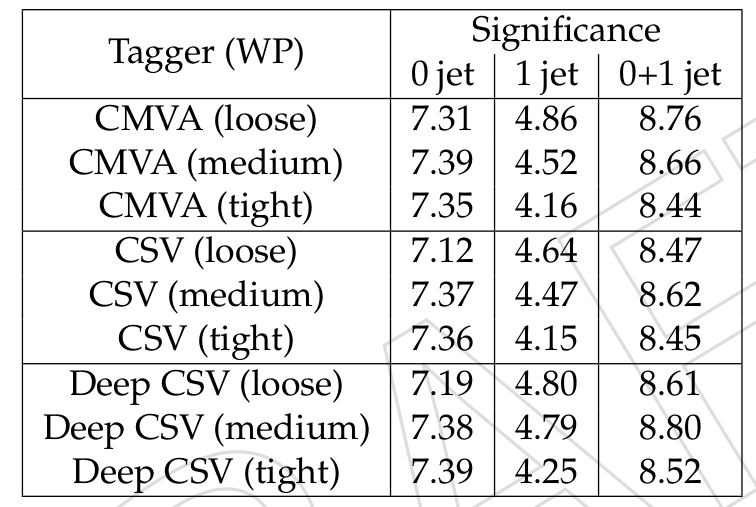
\includegraphics[scale= 0.3]{../Cap4/btt}
\caption{Signal significance for different taggers and working points in the 0 and 1 jet categories. The significance for the combination of the 0 and 1 jet categories is shown as well. Only
the systematic uncertainties associated to the b tagging scale factors are taken into account for
the significance evaluation.}
\label{btt}
\end{figure}

\begin{figure}
\centering
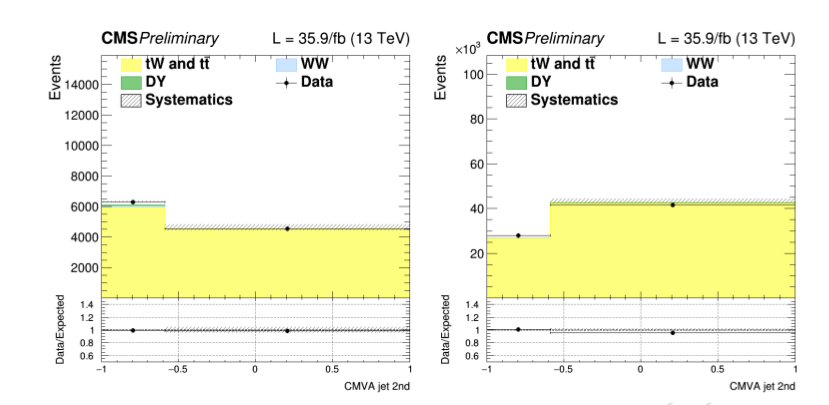
\includegraphics[scale= 0.4]{../Cap4/cmvaT}
\caption{CMVA discriminator for jets above 30 GeV (a) and between 20 and 30 GeV (b) in a
top enriched control region, after applying the scale factors. The top background normalization
is scaled to match data. The systematics band comprises only the uncertainties related to the b
tagging scale factors.}
\label{cmvaT}
\end{figure}

\begin{figure}
\centering
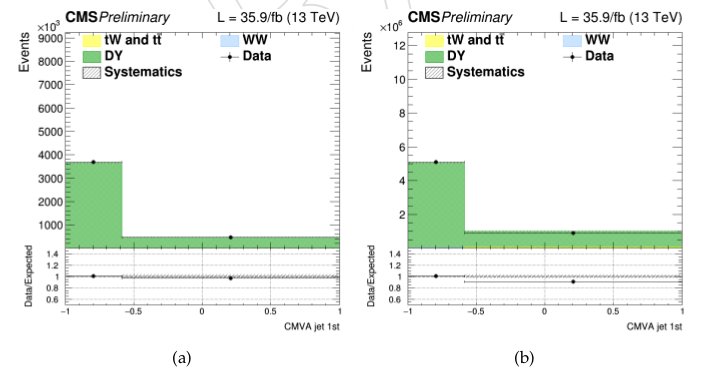
\includegraphics[scale= 0.4]{../Cap4/cmvaD}
\caption{CMVA discriminator for jets between 20 and 30 GeV (a) and above 30 GeV (b) in the
Z enriched control region. The normalization of the DY background is scaled to match data.
The systematics band comprises only the uncertainties related to the b tagging scale factors..}
\label{cmvaD}
\end{figure}

\section{The Missing Transverse Energy}
The longitudinal momentum (along the beam axis) in the collision is not known, so the measurement of the total missing
energy is impossible.
However the initial transverse momentum, carried by the incoming partons, is zero, so in the final state of the collision, for the conservation of the momentum
components, the sum of momenta of all the particles must be zero.
If a missing transverse momentum, $\vec{p_T^{miss}}$, in the transverse plane is present, it is the evidence of invisible particles, such as neutrinos particles predicted by some BSM models.
The $\vec{p_T^{miss}}$ is defined as,
\begin{equation}
\vec{p}_T^{\: miss}= -\sum_{PF\: Objs} \vec{p}_T^{\:PF \: Obj} \: ,
\end{equation}
where the sum extends over all the PF objects. The $\vec{p_T^{miss}}$ is the  negative
vectorial sum of transverse momenta of all reconstructed PF objects, and its module is called missing transverse energy, $E_T^{miss}=|\vec{p_T^{miss}}|$.
As inefficiencies of the tracking algorithm, minimal thresholds in the calorimeter energy
estimation, and nonlinearities of the energy response of the calorimeters for hadronic parti-
cles can introduce a bias in the $\vec{p_T^{miss}}$ determination, a correction is applied by propagating
to the $\vec{p_T^{miss}}$ sum the jet energy corrections,  in according as,
\begin{equation}
\vec{p}_T^{\:miss \: correction}= \vec{p}_T^{\:miss} -\sum_{Jets}( \vec{p}_T^{\:Corr} -\vec{p}_T) \: ,
\end{equation}
where the superscript JEC refers to corrected jets.
To estimate the $E_T^{miss}$  systematic uncertainty we have considered the following sources:
\begin{itemize}
\item jet $p_T$;
\item jet resolution;
\item muon  $p_T$;
\item electron $p_T$;
\item unclustered energy.
\end{itemize}
The $E_T^{miss}$ has been computated varying each of these uncertainties and added in quadrature the
differences with respect to the nominal value. For the $\phi$ uncertainty has been taken as the largest
$\phi$ variation.
The distributions of various  $E_T^{miss}$ variables, in the electron-muon channel, are shown in Fig.~\ref{met}
\begin{figure}
\centering
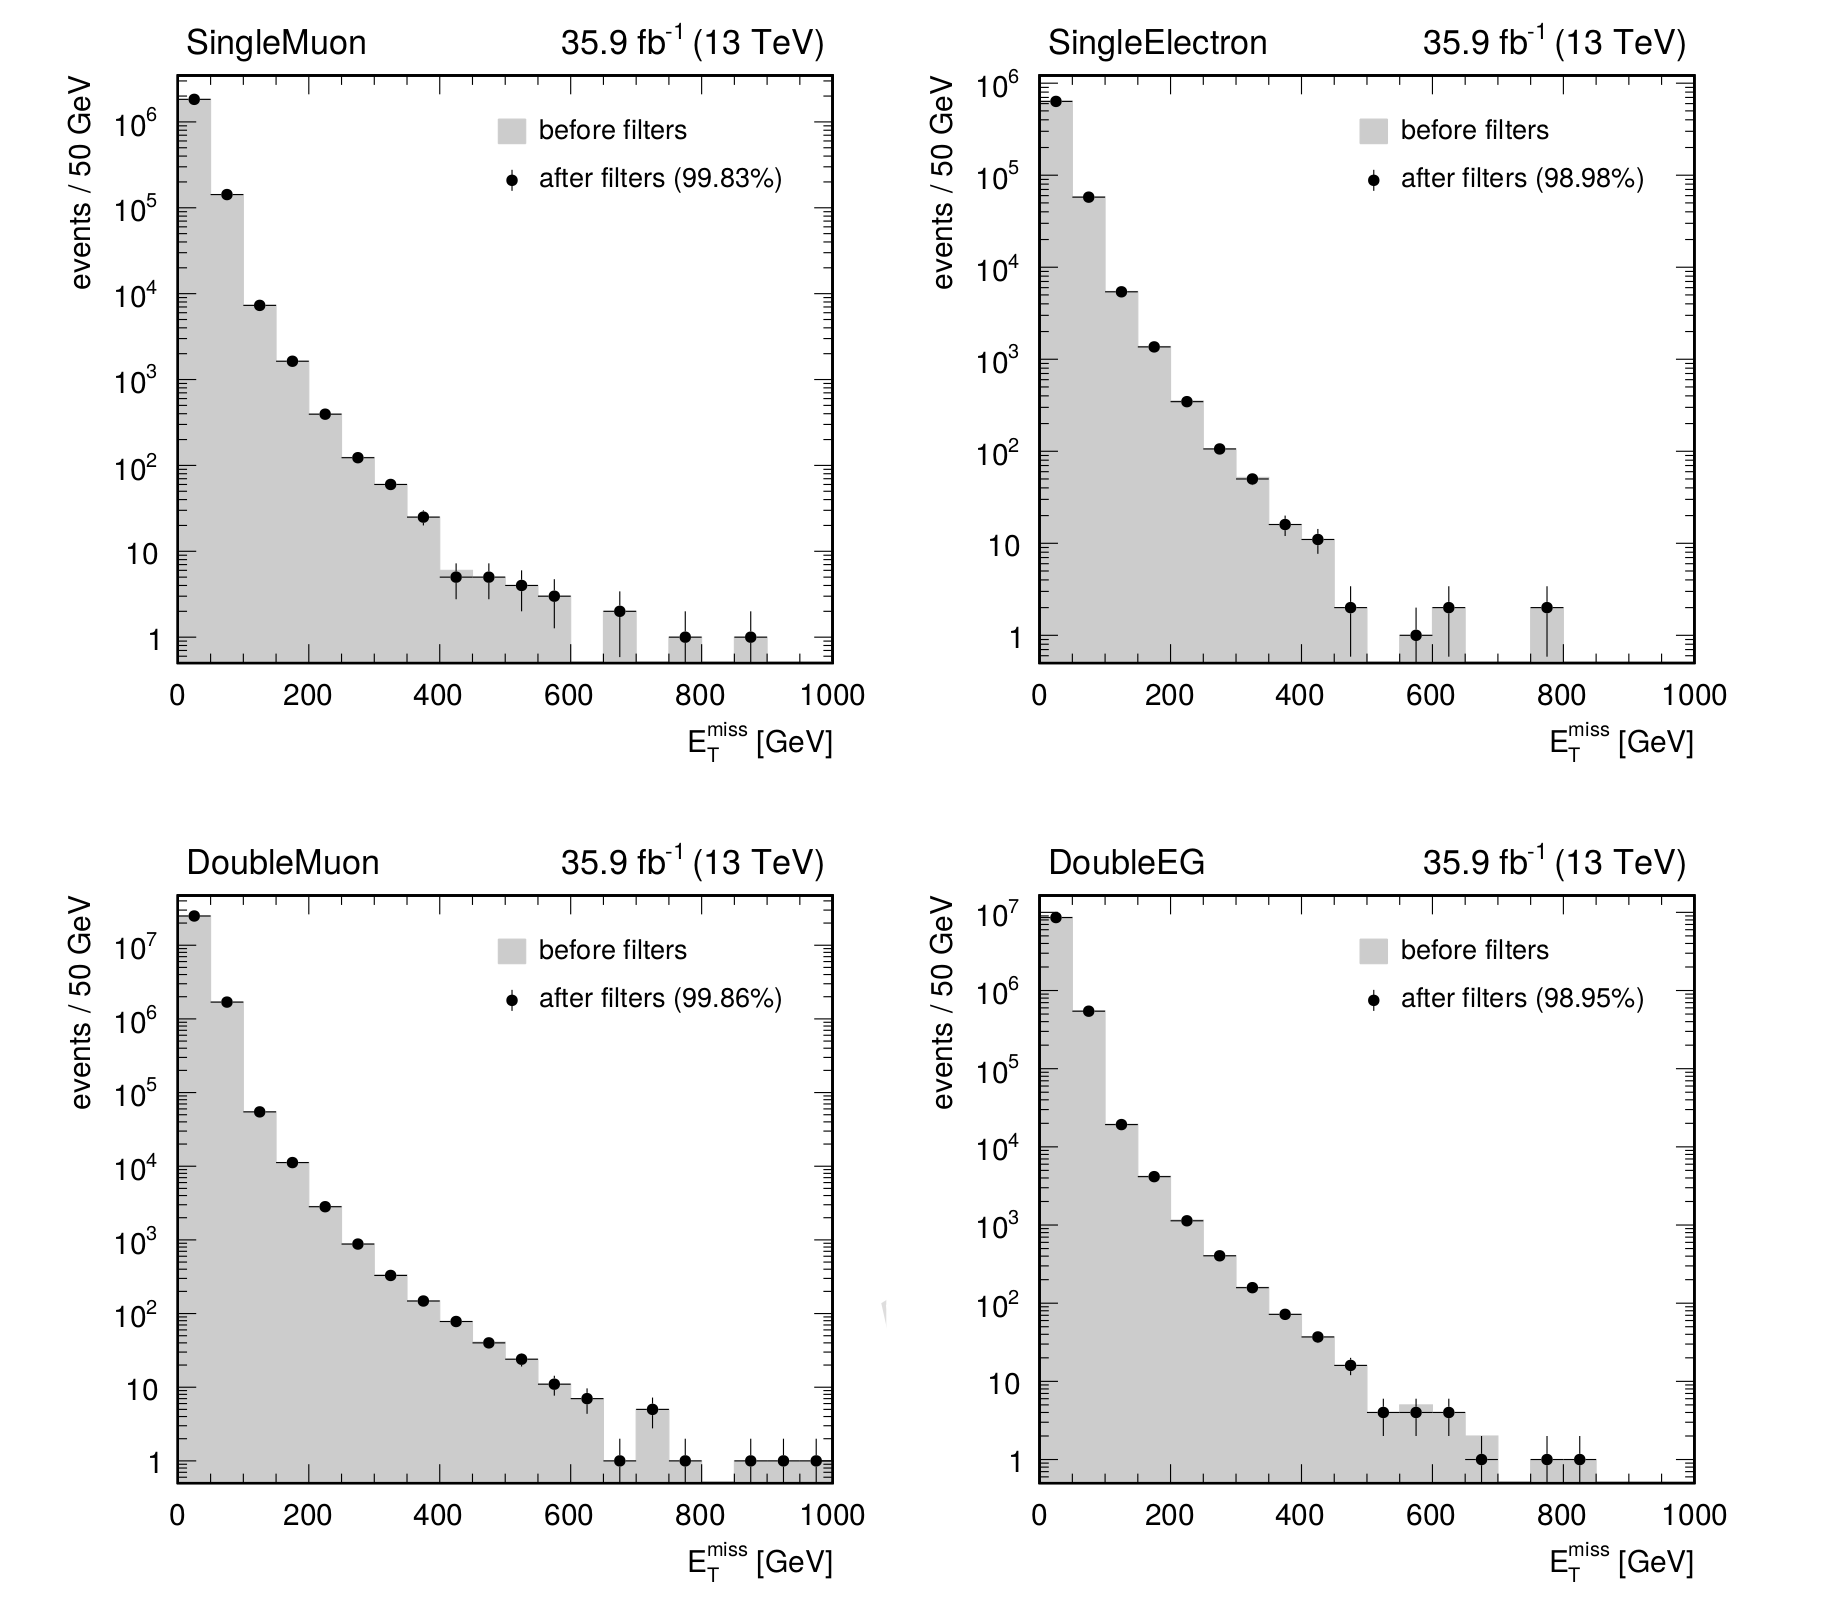
\includegraphics[scale= 0.8]{../Cap4/met}
\caption{The  $E_T^{miss}$ filters efficiencies for 35.9 fb$^{-1}$ of 2016 data. The common requirements for
the distributions before filters (solid histogram) and after filters (black points) are the trigger
and two tight leptons.}
\label{met}
\end{figure}

\section{Fake Lepton Background Estimation}
Lepton fake rates are measured as a
function of the lepton $p_T$ and $\eta$, in a single lepton triggered sample. The test of the method and
systematic errors are described below.
In the analysis
the primary source of background from misidentification is W+Jets. QCD multi-jet and hadronic top backgrounds
are also present at much smaller level. Events in which W bosons are produced in association
with jets give rise to background to WW events when a jet is misidentified as a lepton. These
events contain a real lepton and real missing energy from the W decay. With the jet misidentified 
as a lepton, the W+Jets events have two identified leptons, missing energy, and no other
significant event characteristics. As a result, the W+Jets events cannot be readily suppressed
by event selection. This background is particularly important at low $p_T$.
The estimation of the fake lepton contribution is based on the ``fakeable objet'' data-driven
method and provides a measurement of the yield and the kinematic distributions of fake background. 
It is a general technique, applicable to any physics analysis in which particle level
selection criteria are used to suppress background. The method can be used with any number
of final state particles and is independent of the event selection.
The fundamental idea of the fakeable objet method is simple: select a control sample of events
enriched in the background being estimated, and then use an extrapolation factor to relate these
events to the background in the signal region. The method is data-driven provided the control
sample is selected in data, and the extrapolation factor is measured with data. For background
arising from particle misidentification, the extrapolation is done in particle identification space
($p_T$ and $\eta$ ) of the lepton. The control sample is defined using a looser particle selection criteria
that are chosen such that the rate of misidentification is increased. The extrapolation factor
relates background misidentified with this criteria, to background misidentified as passing the
full particle selection of the signal region.
